% Native PGFPlots; generated by examples/generate_figures.py.
% Constructed or analytical teaching example.
\begingroup
\definecolor{blueplot}{HTML}{4E79A7}
\definecolor{redplot}{HTML}{D95F59}
\definecolor{inkplot}{HTML}{111111}
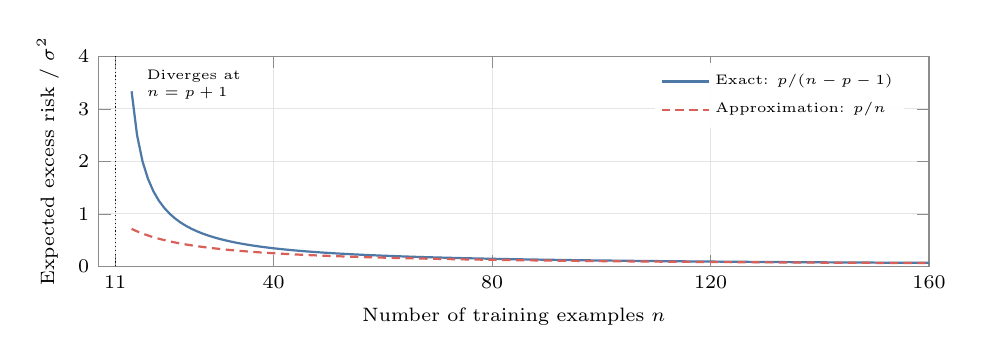
\begin{tikzpicture}
\begin{axis}[
width=\linewidth,height=4.25cm,font=\scriptsize,
tick label style={font=\scriptsize},label style={font=\scriptsize},
axis line style={black!45},tick style={black!45},
grid=major,grid style={black!10},scaled ticks=false,
clip=true,unbounded coords=jump,
legend style={font=\tiny,draw=none,fill=white,fill opacity=.94,text opacity=1,
  legend cell align=left,inner sep=2pt,row sep=1pt},
xmin=8,xmax=160,ymin=0,ymax=4,
xlabel={Number of training examples $n$},ylabel={Expected excess risk / $\sigma^2$},
xtick={11,40,80,120,160},ytick={0,1,2,3,4},legend pos=north east,
]
\addplot[inkplot,densely dotted,forget plot] coordinates {(11,0) (11,4)};
\addplot[blueplot,thick,no marks] coordinates {(14,3.333333333) (15,2.5) (16,2) (17,1.666666667) (18,1.428571429) (19,1.25) (20,1.111111111) (21,1) (22,0.9090909091) (23,0.8333333333) (24,0.7692307692) (25,0.7142857143) (26,0.6666666667) (27,0.625) (28,0.5882352941) (29,0.5555555556) (30,0.5263157895) (31,0.5) (32,0.4761904762) (33,0.4545454545) (34,0.4347826087) (35,0.4166666667) (36,0.4) (37,0.3846153846) (38,0.3703703704) (39,0.3571428571) (40,0.3448275862) (41,0.3333333333) (42,0.3225806452) (43,0.3125) (44,0.303030303) (45,0.2941176471) (46,0.2857142857) (47,0.2777777778) (48,0.2702702703) (49,0.2631578947) (50,0.2564102564) (51,0.25) (52,0.243902439) (53,0.2380952381) (54,0.2325581395) (55,0.2272727273) (56,0.2222222222) (57,0.2173913043) (58,0.2127659574) (59,0.2083333333) (60,0.2040816327) (61,0.2) (62,0.1960784314) (63,0.1923076923) (64,0.1886792453) (65,0.1851851852) (66,0.1818181818) (67,0.1785714286) (68,0.1754385965) (69,0.1724137931) (70,0.1694915254) (71,0.1666666667) (72,0.1639344262) (73,0.1612903226) (74,0.1587301587) (75,0.15625) (76,0.1538461538) (77,0.1515151515) (78,0.1492537313) (79,0.1470588235) (80,0.1449275362) (81,0.1428571429) (82,0.1408450704) (83,0.1388888889) (84,0.1369863014) (85,0.1351351351) (86,0.1333333333) (87,0.1315789474) (88,0.1298701299) (89,0.1282051282) (90,0.1265822785) (91,0.125) (92,0.1234567901) (93,0.1219512195) (94,0.1204819277) (95,0.119047619) (96,0.1176470588) (97,0.1162790698) (98,0.1149425287) (99,0.1136363636) (100,0.1123595506) (101,0.1111111111) (102,0.1098901099) (103,0.1086956522) (104,0.1075268817) (105,0.1063829787) (106,0.1052631579) (107,0.1041666667) (108,0.1030927835) (109,0.1020408163) (110,0.101010101) (111,0.1) (112,0.09900990099) (113,0.09803921569) (114,0.09708737864) (115,0.09615384615) (116,0.09523809524) (117,0.09433962264) (118,0.09345794393) (119,0.09259259259) (120,0.09174311927) (121,0.09090909091) (122,0.09009009009) (123,0.08928571429) (124,0.08849557522) (125,0.08771929825) (126,0.08695652174) (127,0.08620689655) (128,0.08547008547) (129,0.08474576271) (130,0.08403361345) (131,0.08333333333) (132,0.0826446281) (133,0.08196721311) (134,0.08130081301) (135,0.08064516129) (136,0.08) (137,0.07936507937) (138,0.07874015748) (139,0.078125) (140,0.07751937984) (141,0.07692307692) (142,0.07633587786) (143,0.07575757576) (144,0.07518796992) (145,0.07462686567) (146,0.07407407407) (147,0.07352941176) (148,0.07299270073) (149,0.07246376812) (150,0.07194244604) (151,0.07142857143) (152,0.07092198582) (153,0.07042253521) (154,0.06993006993) (155,0.06944444444) (156,0.06896551724) (157,0.06849315068) (158,0.06802721088) (159,0.06756756757) (160,0.06711409396)};
\addlegendentry{Exact: $p/(n-p-1)$}
\addplot[redplot,thick,densely dashed,no marks] coordinates {(14,0.7142857143) (15,0.6666666667) (16,0.625) (17,0.5882352941) (18,0.5555555556) (19,0.5263157895) (20,0.5) (21,0.4761904762) (22,0.4545454545) (23,0.4347826087) (24,0.4166666667) (25,0.4) (26,0.3846153846) (27,0.3703703704) (28,0.3571428571) (29,0.3448275862) (30,0.3333333333) (31,0.3225806452) (32,0.3125) (33,0.303030303) (34,0.2941176471) (35,0.2857142857) (36,0.2777777778) (37,0.2702702703) (38,0.2631578947) (39,0.2564102564) (40,0.25) (41,0.243902439) (42,0.2380952381) (43,0.2325581395) (44,0.2272727273) (45,0.2222222222) (46,0.2173913043) (47,0.2127659574) (48,0.2083333333) (49,0.2040816327) (50,0.2) (51,0.1960784314) (52,0.1923076923) (53,0.1886792453) (54,0.1851851852) (55,0.1818181818) (56,0.1785714286) (57,0.1754385965) (58,0.1724137931) (59,0.1694915254) (60,0.1666666667) (61,0.1639344262) (62,0.1612903226) (63,0.1587301587) (64,0.15625) (65,0.1538461538) (66,0.1515151515) (67,0.1492537313) (68,0.1470588235) (69,0.1449275362) (70,0.1428571429) (71,0.1408450704) (72,0.1388888889) (73,0.1369863014) (74,0.1351351351) (75,0.1333333333) (76,0.1315789474) (77,0.1298701299) (78,0.1282051282) (79,0.1265822785) (80,0.125) (81,0.1234567901) (82,0.1219512195) (83,0.1204819277) (84,0.119047619) (85,0.1176470588) (86,0.1162790698) (87,0.1149425287) (88,0.1136363636) (89,0.1123595506) (90,0.1111111111) (91,0.1098901099) (92,0.1086956522) (93,0.1075268817) (94,0.1063829787) (95,0.1052631579) (96,0.1041666667) (97,0.1030927835) (98,0.1020408163) (99,0.101010101) (100,0.1) (101,0.09900990099) (102,0.09803921569) (103,0.09708737864) (104,0.09615384615) (105,0.09523809524) (106,0.09433962264) (107,0.09345794393) (108,0.09259259259) (109,0.09174311927) (110,0.09090909091) (111,0.09009009009) (112,0.08928571429) (113,0.08849557522) (114,0.08771929825) (115,0.08695652174) (116,0.08620689655) (117,0.08547008547) (118,0.08474576271) (119,0.08403361345) (120,0.08333333333) (121,0.0826446281) (122,0.08196721311) (123,0.08130081301) (124,0.08064516129) (125,0.08) (126,0.07936507937) (127,0.07874015748) (128,0.078125) (129,0.07751937984) (130,0.07692307692) (131,0.07633587786) (132,0.07575757576) (133,0.07518796992) (134,0.07462686567) (135,0.07407407407) (136,0.07352941176) (137,0.07299270073) (138,0.07246376812) (139,0.07194244604) (140,0.07142857143) (141,0.07092198582) (142,0.07042253521) (143,0.06993006993) (144,0.06944444444) (145,0.06896551724) (146,0.06849315068) (147,0.06802721088) (148,0.06756756757) (149,0.06711409396) (150,0.06666666667) (151,0.06622516556) (152,0.06578947368) (153,0.06535947712) (154,0.06493506494) (155,0.06451612903) (156,0.0641025641) (157,0.06369426752) (158,0.06329113924) (159,0.06289308176) (160,0.0625)};
\addlegendentry{Approximation: $p/n$}
\node[font=\tiny,anchor=north west,align=left] at (axis cs:15,3.92) {Diverges at\\$n=p+1$};

\end{axis}
\end{tikzpicture}
\endgroup
